\documentclass[11pt,a4paper]{article}
\usepackage[utf8]{inputenc}
\usepackage[T1]{fontenc}
\usepackage{amsmath}
\usepackage{amsfonts}
\usepackage{amssymb}
\usepackage{graphicx,fullpage}
\usepackage{listings}
\usepackage{color}



\definecolor{dkgreen}{rgb}{0,0.6,0}
\definecolor{gray}{rgb}{0.5,0.5,0.5}
\definecolor{mauve}{rgb}{0.58,0,0.82}

\lstset{frame=tb,
	language=R,
	aboveskip=3mm,
	belowskip=3mm,
	showstringspaces=false,
	columns=flexible,
	basicstyle={\small\ttfamily},
	numbers=none,
	numberstyle=\tiny\color{gray},
	keywordstyle=\color{blue},
	commentstyle=\color{dkgreen},
	stringstyle=\color{mauve},
	breaklines=true,
	breakatwhitespace=true,
	tabsize=3
}


\begin{document}
	\title{\textbf{Time series analysis of Crude Oil Prices}}
	\author{Hemanthkumar E (19BM6JP27)\and
		Mudigal Murali Krishna (19BM6JP29) \and 
		Paturu Harish (19BM6JP55) \and 
		Venkata Satya Sai Andhavarapu (19BM6JP61) \and 
		Vineet Kumar (19BM6JP46)
	}
\date{\today\thanks{Submitted as course project report of RTSM 2020 taught at IIT Kharagpur. Names appear in alphabetical order.}}
\maketitle
\begin{abstract}
	In this work we aim to examine modeling crude oil prices from publicly available historical time series data. The oil prices are very diffcult to model given their complex and non linear behaviour. 
\end{abstract}
\maketitle
\section{Introduction}
 
Time series is a stochastic process with continuous random variables and time as an index which is discrete. So, it is a series of data points indexed in time order generally at successive equal intervals of discrete-time points.

Time Series Analysis accounts for the fact that data points taken over time may have an internal structure or pattern (such as autocorrelation, trend or seasonal variation) that should be accounted for. So, to understand such patterns, it is possible in principle to apply basic modern mathematical tools and techniques such as MA, AR,ARMA,ARIMA (popularly known as Box-Jenkins methodologies) and SARIMA which integrates the seasonal component to forecast the future values.


The aim of the project is to identify a model best fitting the Crude Oil Prices data to forecast the future price.The properties of the data are described and basic time series techniques are applied to the data. Plots of the series, autocorrelation function and the partial autocorrelation function are some of the graphical tools used to analyze the series. Different models have been fitted to the data in order to make credible forecasts from the model.

\section{Background \& Model Description}

\begin{itemize}
	\item AR model: Autoregressive models of order p ,abbreviated AR(p), is one of the commonly used time series models. In the AR model the current observations depend on the level of its lagged observations. 
	
	\item MA Model: Moving average model of order q,abbreviated MA(q), models the current observations depend on the error term of  lagged observations. 
	
	\item ARMA model: ARMA model is made up of two processes namely the Autoregressive(AR) and the Moving Average(MA).
	
	\item ARIMA: AutoRegressive Integrated Moving Average models intend to describe the current
	behavior of variables in terms of linear relationships with their past values. It has an
	Integrated (I) component (d), which represents the amount of differencing to be performed
	on the series to make it stationary. The second component of the ARIMA consists of an
	ARMA model for the series rendered stationary through differentiation. The ARMA
	component is further decomposed into AR and MA components which are explained
	above. The Autocorrelation Function (ACF) and Partial Autocorrelation Function (PACF) are
	used to estimate the values of the orders of the AR and MA processes respectively. The
	statistical package R is used to analyze the data.
	
	\item SARIMA: Seasonal ARIMA is similar to the ARIMA model in which seasonal components are also considered.
	
	
	
\end{itemize}
\section{Data Description \& EDA}

\subsection{Data Source}

“Crude oil prices daily” is the dataset used which is obtained from the Kaggle dataset repository with the usability index 4.7 and licensed under GPL2. The dataset consists of two to columns namely date column  and corresponding crude oil price in dollars.The data has been recorded from 1986 to 2018 with 8223 data points. Additional datasets which represent macro\_economic trends like Dollar-Yen exchange rates, Dollar-Yuan exchange rates, Pound-Dollar exchange rates which might impact the crude oil price are considered.


The descriptive statistics of crude oil prices were analyzed by  as mean, standard deviation, skewness, kurtosis etc. They are shown is Table: 1.

	\begin{table}[h!]
	\begin{center}
\begin{tabular}{c c c c c }
	\hline
mean	& median & std. deviation  & skewness & kurtosis \\
	\hline
62.06077	& 58.9800 & 27.10157 & 0.3588734 & 2.146504\\
	\hline
\end{tabular}\end{center}
	\label{desc}
	\caption{Descriptive Statistics}
\end{table}


Above measures evidently shows the \textbf{complex nonlinear dynamic} data features in the crude oil price data, whose distribution \underline{significantly deviates from normal distribution}. 
Non zero kurtosis means tendency to produce outliers \cite{westfall2014kurtosis}. The significant kurtosis value indicates the probability of extreme event occurrence.



\subsection{Handling Missing Values} 
Our data had 7 missing values. We imputed them using last observation value. 
\begin{lstlisting}
length(price[is.na(price)])  ## no. of missing values
## imputing missing values using last observation ####
dat=na.locf(price, option = "nocb")
\end{lstlisting}


\begin{figure}[h!]
	\centering
	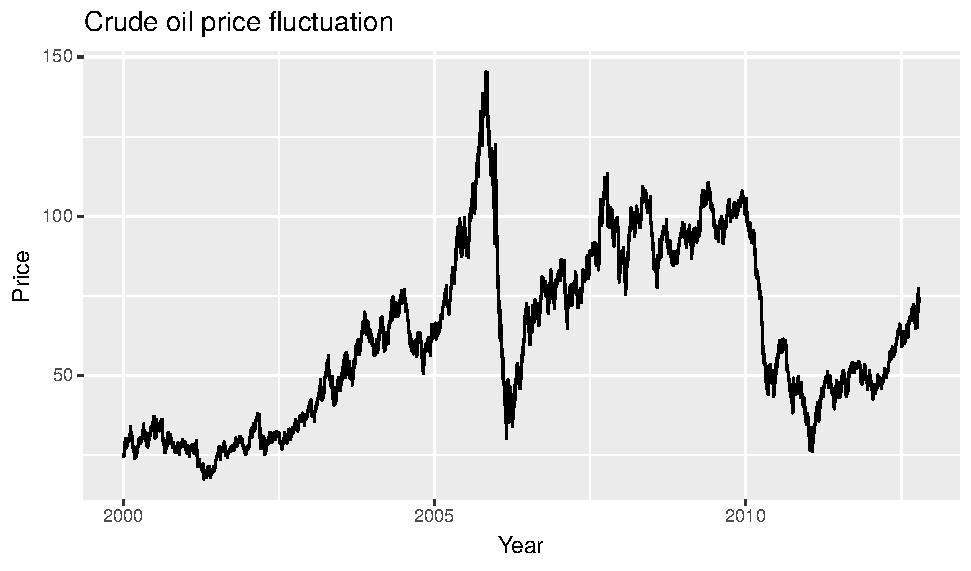
\includegraphics[width=0.7\linewidth]{../Oil-Price-Forecasting/crude}
	\caption{Time Series Data of Crude Oil Price}
	\label{fig:crude}
\end{figure}
\pagebreak
Now, let us have a look at yearly price fluctuation.
\begin{figure}[h!]
	\centering
	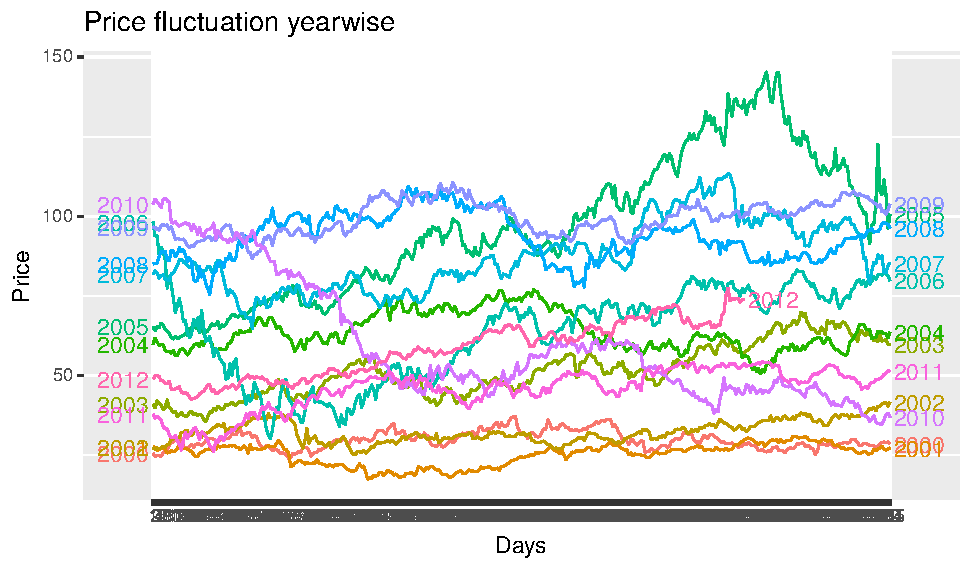
\includegraphics[width=0.7\linewidth]{../Oil-Price-Forecasting/price}
	\caption{Yearly Price Fluctuations}
	\label{fig:price}
\end{figure}

Another way to look at time series data is to plot each observation against another observation that occurred some time previously. This is called a lag plot because we are plotting the time series against lags of itself. 

\begin{figure}[h!]
	\centering
	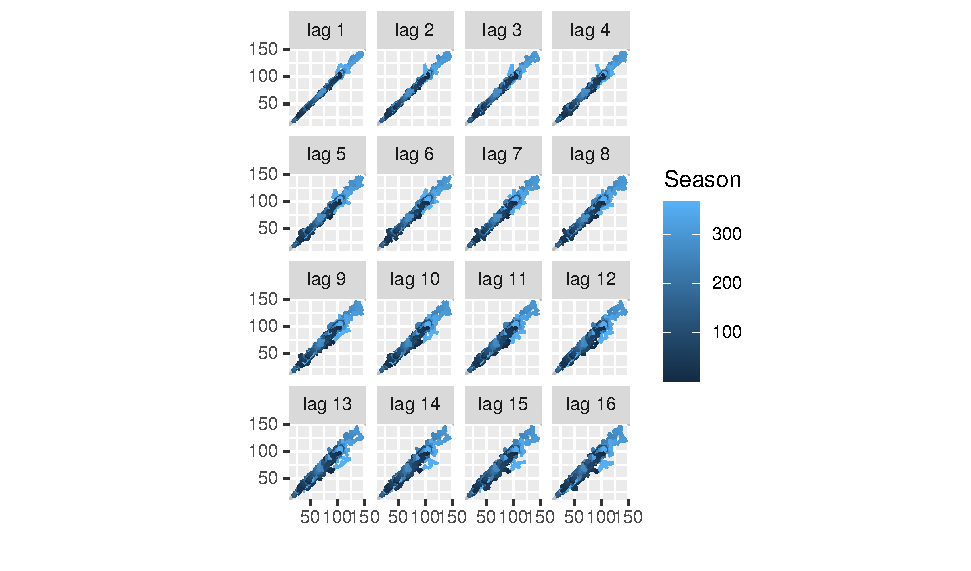
\includegraphics[width=0.9\linewidth]{../Oil-Price-Forecasting/lag}
	\caption{Lag Plot}
	\label{fig:lag}
\end{figure}

The random fluctuations in the time series do not appear to be constant in size over time, so it is probably appropriate to describe the data using a \underline{multiplicative} model. The multiplicative decomposition of time series is shown below
\begin{figure}
	\centering
	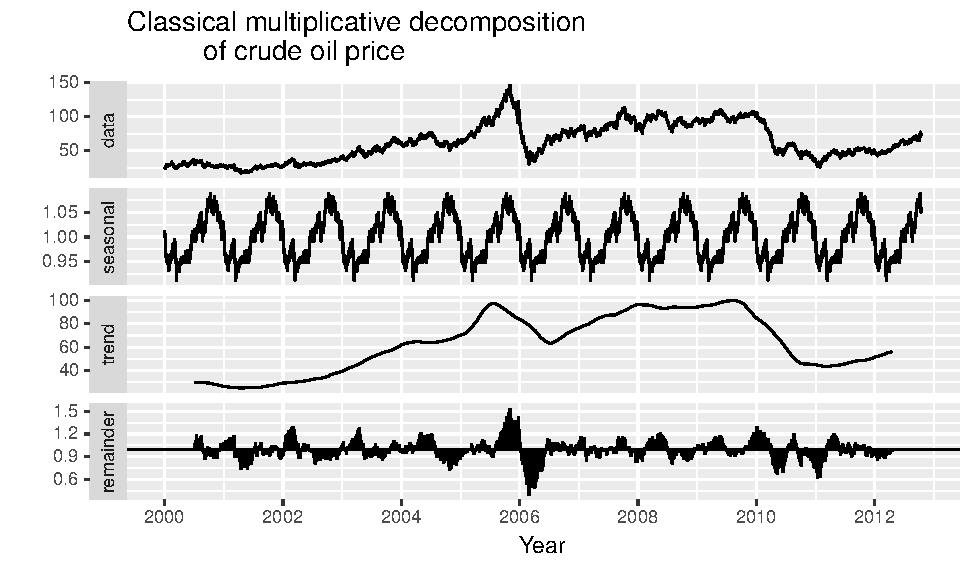
\includegraphics[width=0.7\linewidth]{../Oil-Price-Forecasting/decomposition}
	\caption{Multiplicative Decomposition}
	\label{fig:decomposition}
\end{figure}

\subsection{Testing Normality Assumption}
\begin{lstlisting}
jarque.test(dat$Closing.Value)

Jarque-Bera Normality Test

data:  dat$Closing.Value
JB = 242.14, p-value < 2.2e-16
alternative hypothesis: greater

\end{lstlisting}
The p-value is \textbf{less than 0.05} cutoff value for JB test. This indicates that the distribution of the crude oil price movement \textbf{does not conform to the normal distribution} and the crude oil price movement \textit{may} contain nonlinear dependence in data.

\subsection{Testing Stationarity}
\paragraph{Augmented Dickey–Fuller (ADF)} tests the null hypothesis that a unit root is present in a data. 
The null hypothesis for both tests is that the data are non-stationary. We want to REJECT the null hypothesis for this test, so we want a p-value of less that 0.05 (or smaller).

Transformations such as logarithms can help to stabilise the variance of a time series. Differencing can help stabilise the mean of a time series by removing changes in the level of a time series, and therefore eliminating (or reducing) trend and seasonality.

\begin{lstlisting}

tseries::adf.test(train)

Augmented Dickey-Fuller Test

data:  train
Dickey-Fuller = -1.9507, Lag order = 16, p-value = 0.5992
alternative hypothesis: stationary


\end{lstlisting}
Our time series is non-stationary. To make it stationary we took the first difference. 
\begin{lstlisting}
> tr_diff<-diff(train)
> tseries::adf.test(tr_diff)

Augmented Dickey-Fuller Test

data:  tr_diff
Dickey-Fuller = -15.623, Lag order = 16, p-value = 0.01
alternative hypothesis: stationary

\end{lstlisting}

Now our time series is \textbf{stationary}, as clearly evident from the below figure.
\begin{figure}[h!]
	\centering
	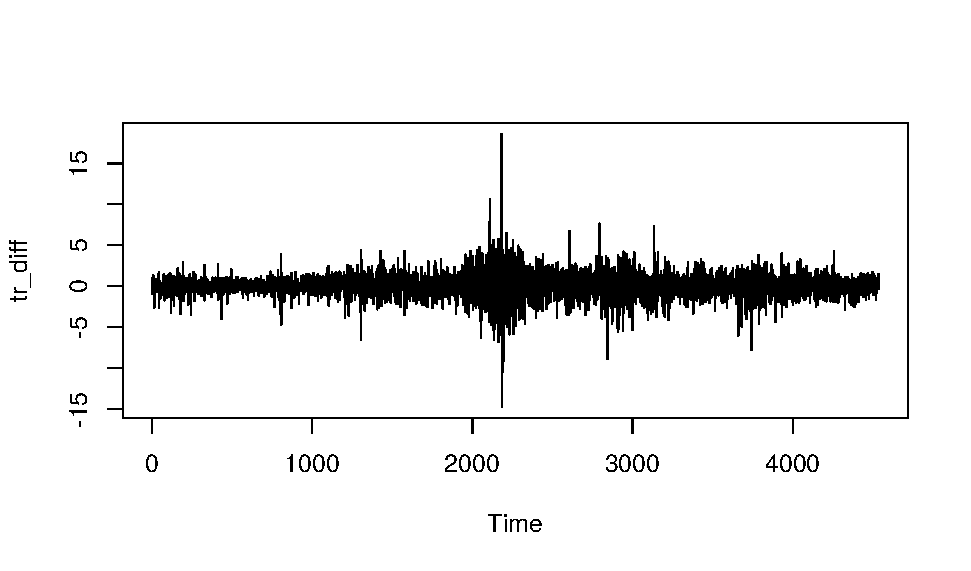
\includegraphics[width=0.7\linewidth]{../Oil-Price-Forecasting/first-diff}
	\caption{First Difference Stationary}
	\label{fig:first-diff}
\end{figure}




\section{Model Analysis}
We experimented with some simple as well as complex models.
\subsection{Exponential Smoothing}
Exponential smoothing schemes weight past observations using exponentially decreasing weights. This is a very popular scheme to produce a smoothed Time Series. Exponential Smoothing assigns exponentially decreasing weights as the observation get older.
	
\begin{figure}[h!]
	\centering
	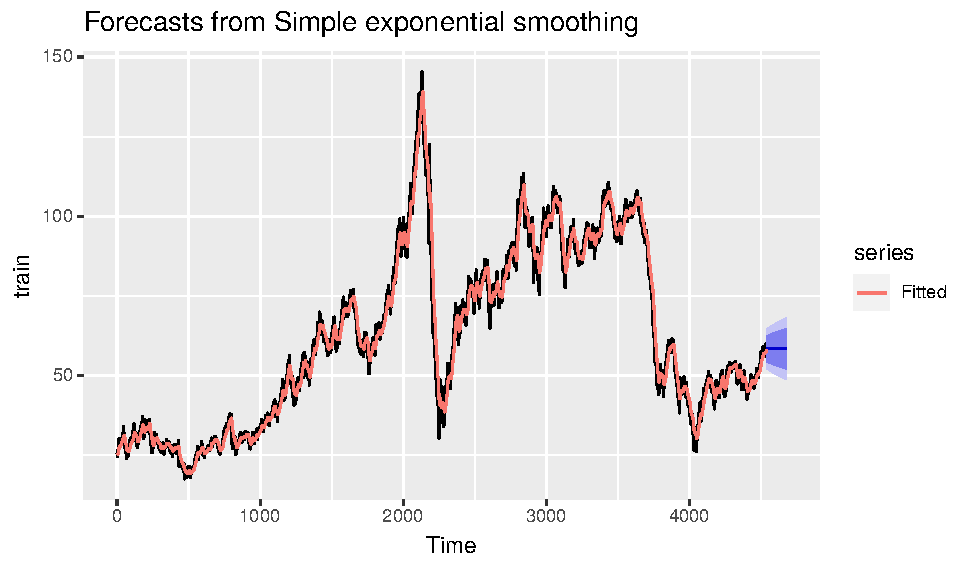
\includegraphics[width=0.7\linewidth]{../Oil-Price-Forecasting/exp}
	\caption{Forecast of Exponential Smoothing Model}
	\label{fig:exp}
\end{figure}

\subsubsection{HoltWinters}

The Holt-Winters seasonal method comprises the forecast equation and three smoothing equations — one for the level  
$l_t$
, one for the trend  
$b_t$
, and one for the seasonal component  
$s_t$
, with corresponding smoothing parameters  
$\alpha$
,  
$\beta$
and  
$\gamma$
. We use  
$m$
to denote the frequency of the seasonality. The component form for the multiplicative method is:

\begin{align*}
\hat{y}_{t+h|t} &= (\ell_{t} + hb_{t})s_{t+h-m(k+1)} \\
\ell_{t} &= \alpha \frac{y_{t}}{s_{t-m}} + (1 - \alpha)(\ell_{t-1} + b_{t-1})\\
b_{t} &= \beta^*(\ell_{t}-\ell_{t-1}) + (1 - \beta^*)b_{t-1}                \\
s_{t} &= \gamma \frac{y_{t}}{(\ell_{t-1} + b_{t-1})} + (1 - \gamma)s_{t-m}
\end{align*}


\begin{lstlisting}
> trainforecasts <- HoltWinters(train, gamma=FALSE)
> trainforecasts
Holt-Winters exponential smoothing with trend and without seasonal component.

Call:
HoltWinters(x = train, gamma = FALSE)

Smoothing parameters:
alpha: 0.9432677
beta : 0.01343652
gamma: FALSE

Coefficients:
[,1]
a 60.3922357
b  0.1016818
> plot(trainforecasts)

\end{lstlisting}
\begin{figure}[h!]
	\centering
	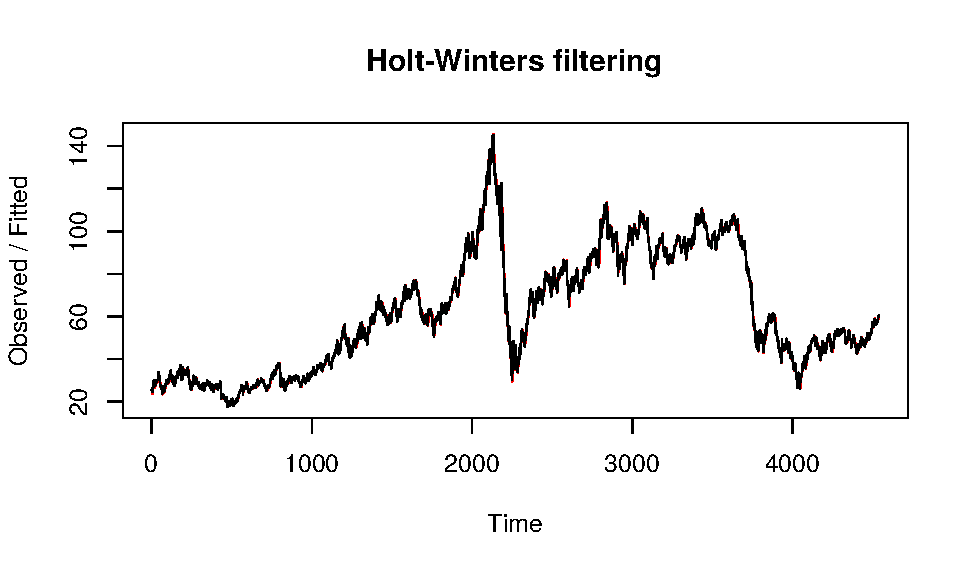
\includegraphics[width=0.9\linewidth]{../Oil-Price-Forecasting/holt}
	\caption{Holt Winters Smoothing}
	\label{fig:holt}
\end{figure}
\subsubsection*{Interpretation of $\alpha, \beta,  \and \gamma $}
\paragraph{alpha}This is also known as the base value. This value determines the weighting of past data values in setting the baseline (magnitude) for the forecast, with higher values of Alpha leading to the increased weight being given to the most recent observations, while lower values of Alpha implying a more uniform weighting

\paragraph{beta} This is also known as the trend value. It determines the degree to which recent data trends should be valued compared to older trends when making the forecast.
\paragraph{gamma} This is the seasonal component of the forecast, and the higher the parameter, the more the recent seasonal component is weighed. The seasonal component is the repeating pattern of the forecast.

In our case \underline{alpha is  high}, telling us that the \textbf{estimate of the current value of the level is mostly upon very recent observations} in the time series. This makes good intuitive sense, since the level and the slope of the time series both change quite a lot over time. 



\subsection{Moving Average}
In Single Moving Averages the past observations are weighted equally.
Moving average model of order $q$, abbreviated $MA(q)$, models the current observations depend on the error term of  lagged observations. 

\begin{figure}[h!]
	\centering
	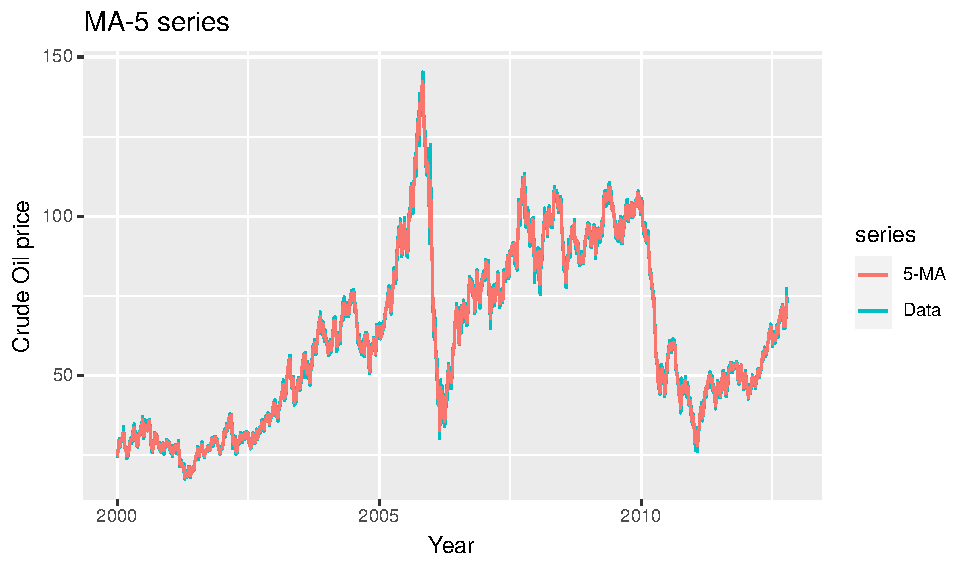
\includegraphics[width=0.7\linewidth]{../Oil-Price-Forecasting/ma}
	\caption{MA(5) fitting}
	\label{fig:ma}
\end{figure}


\subsection{ARIMA}
 AutoRegressive Integrated Moving Average models intend to describe the current
behavior of variables in terms of linear relationships with their past values. It has an
Integrated $(I)$ component $(d)$, which represents the amount of differencing to be performed
on the series to make it stationary. 
\begin{lstlisting}
> fit<-auto.arima(train, stepwise = FALSE)
> fc=forecast(fit,h=136)
> summary(fit)
Series: train 
ARIMA(0,1,5) 

Coefficients:
ma1      ma2     ma3     ma4      ma5
-0.0492  -0.0205  0.0293  0.0224  -0.0481
s.e.   0.0148   0.0148  0.0147  0.0151   0.0147

sigma^2 estimated as 2.089:  log likelihood=-8104.71
AIC=16221.42   AICc=16221.44   BIC=16259.94

Training set error measures:
ME     RMSE       MAE         MPE     MAPE      MASE          ACF1
Training set 0.008214873 1.444411 0.9998611 -0.01165554 1.753502 0.9981886 -0.0006202995

\end{lstlisting}

\begin{figure}[h!]
	\centering
	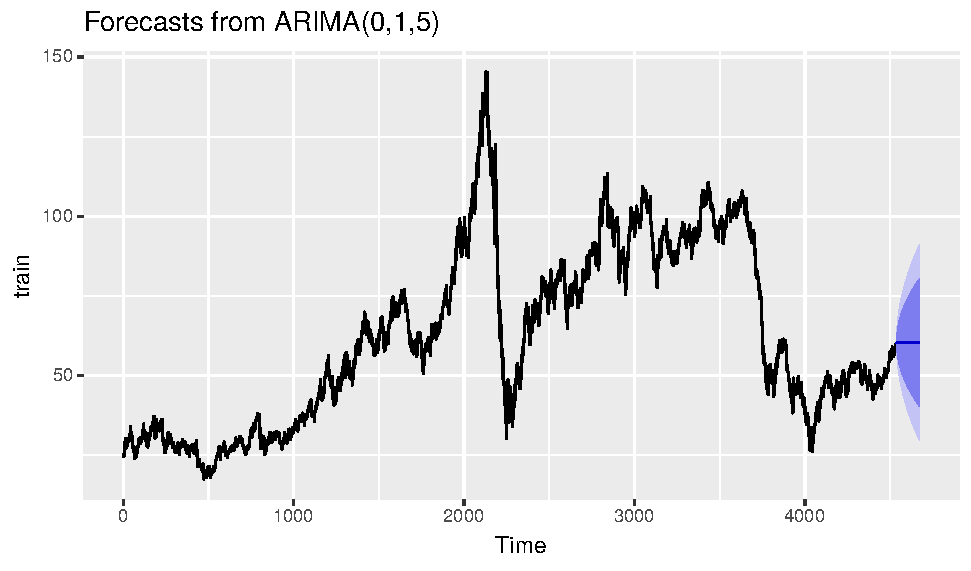
\includegraphics[width=0.9\linewidth]{../Oil-Price-Forecasting/arima}
	\caption{ARIMA}
	\label{fig:arima}
\end{figure}
Examining the residuals we observed from the ACF plot that there is significant correlation in residuals. Residuals are not white noise.

\begin{figure}[h!]
	\centering
	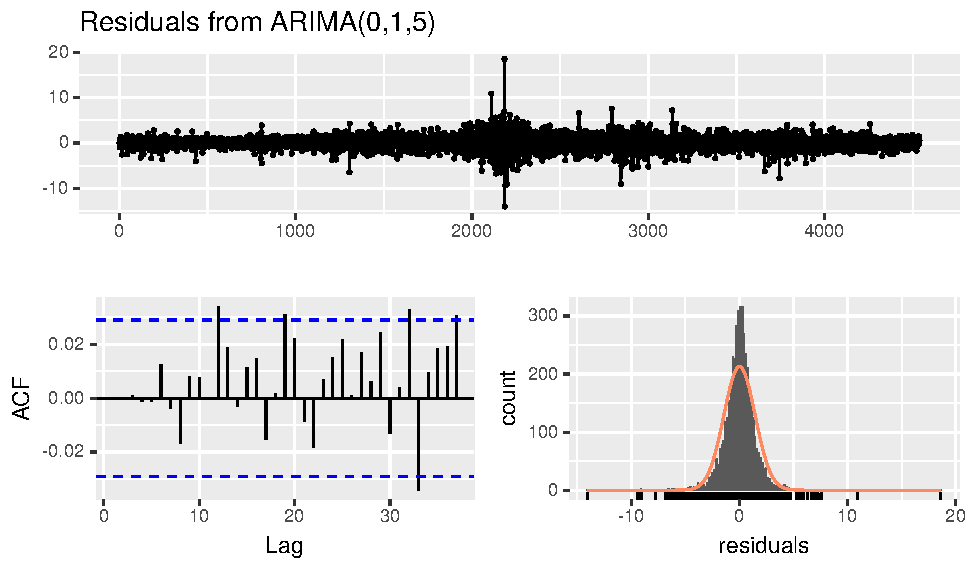
\includegraphics[width=0.9\linewidth]{../Oil-Price-Forecasting/arma-res}
	\caption{Residuals of ARIMA}
	\label{fig:arma-res}
\end{figure}

\begin{lstlisting}
> checkresiduals(fit)
Ljung-Box test

data:  Residuals from ARIMA(0,1,5)
Q* = 2.6876, df = 5, p-value = 0.748

Model df: 5.   Total lags used: 10
\end{lstlisting}
\pagebreak
\subsection{Seasonal ARIMA}


\begin{lstlisting}
> ### Applying SARIMA ###
> fit_s<-auto.arima(train,  seasonal = T,stepwise = FALSE)
> fc_s=forecast(fit_s,h=136)
> ## summary of the model ####
> ## No seasonality found
> summary(fit_s)
Series: train 
ARIMA(0,1,5) 

Coefficients:
ma1      ma2     ma3     ma4      ma5
-0.0492  -0.0205  0.0293  0.0224  -0.0481
s.e.   0.0148   0.0148  0.0147  0.0151   0.0147

sigma^2 estimated as 2.089:  log likelihood=-8104.71
AIC=16221.42   AICc=16221.44   BIC=16259.94

Training set error measures:
ME     RMSE       MAE         MPE     MAPE      MASE          ACF1
Training set 0.008214873 1.444411 0.9998611 -0.01165554 1.753502 0.9981886 -0.0006202995

\end{lstlisting}

\begin{figure}[h!]
	\centering
	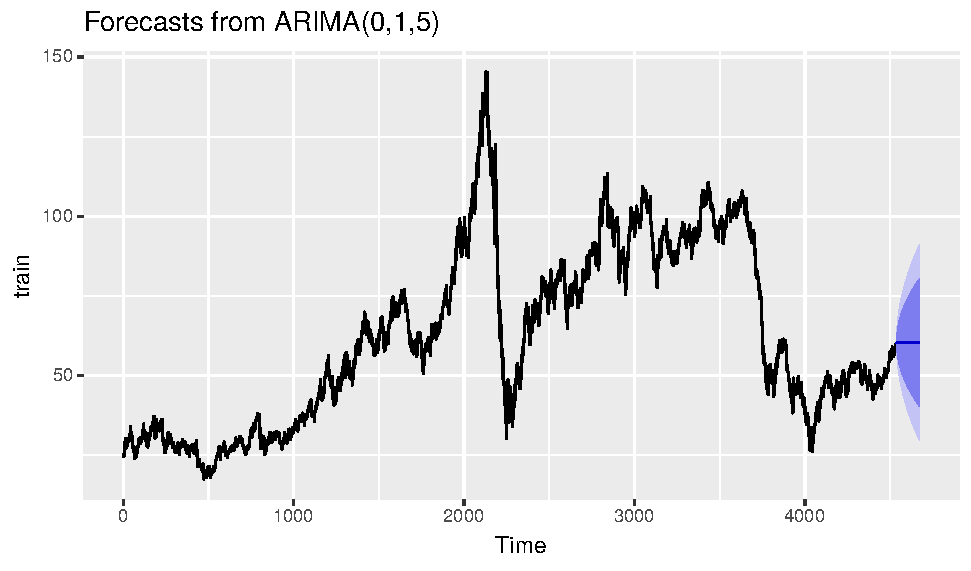
\includegraphics[width=0.7\linewidth]{../Oil-Price-Forecasting/sarima}
	\caption{Seasonal ARIMA fit}
	\label{fig:sarima}
\end{figure}
No seasonality found in out data. 


Simpler models are quite successful in numerous applications, they are unable to represent many non-linear dynamic patterns. It would not be reasonable to expect a single, linear model to capture these distinct behaviours.\cite{chen2017forecasting}

\subsection{TBATS for multiple seasonality}

\begin{lstlisting}

fit_t= tbats(train)

fc_t=forecast(fit_t,h=136)

### summary ###

summary(fit_t)
Length Class  Mode     
lambda               1   -none- numeric  
alpha                1   -none- numeric  
beta                 0   -none- NULL     
damping.parameter    0   -none- NULL     
gamma.values         0   -none- NULL     
ar.coefficients      0   -none- NULL     
ma.coefficients      0   -none- NULL     
likelihood           1   -none- numeric  
optim.return.code    1   -none- numeric  
variance             1   -none- numeric  
AIC                  1   -none- numeric  
parameters           2   -none- list     
seed.states          1   -none- numeric  
fitted.values     4537   -none- numeric  
errors            4537   -none- numeric  
x                 4537   -none- numeric  
seasonal.periods     0   -none- NULL     
y                 4537   -none- numeric  
call                 2   -none- call     
series               1   -none- character
method               1   -none- character

\end{lstlisting}
\begin{figure}[h!]
	\centering
	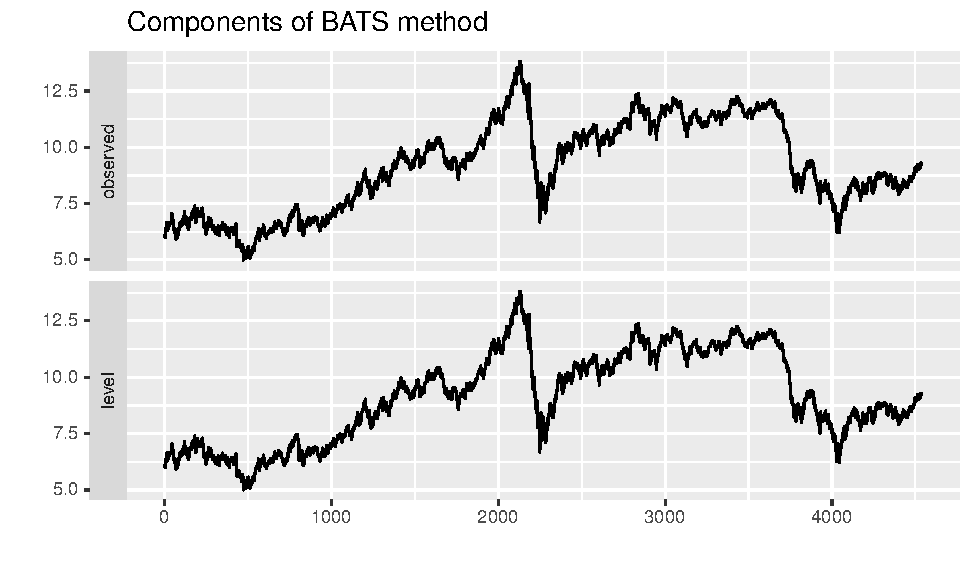
\includegraphics[width=0.7\linewidth]{../Oil-Price-Forecasting/bats}
	\caption{T-BATS Model}
	\label{fig:bats}
\end{figure}

\subsection{Additive nonlinear autoregressive model}
In time series modeling, a nonlinear autoregressive exogenous model  is a nonlinear autoregressive model which has exogenous inputs. 

\begin{figure}[h!]
	\centering
	\includegraphics[width=0.7\linewidth]{../Oil-Price-Forecasting/aar1}
	\caption{AAR Model Fit}
	\label{fig:aar1}
\end{figure}


\begin{figure}[h!]
	\centering
	\includegraphics[width=0.46\linewidth]{../Oil-Price-Forecasting/aar2}
	\includegraphics[width=0.46\linewidth]{../Oil-Price-Forecasting/aar3}
	\caption{AAR ACF \& PACF Plots}
	\label{fig:aar2}
\end{figure}

\begin{lstlisting}
> res.mod<-predict_rolling(mod, newdata=test)
> accuracy_stat(res.mod)
var         ME     RMSE       MAE       MPE     MAPE
x   x 0.08865304 1.130757 0.8038681 0.1178298 1.213731

\end{lstlisting}
\subsection{GARCH}
 Generalized autoregressive conditional heteroskedasticity model, abbreviated $GARCH(p, q)$, is an $ARMA(p,q)$ model applied to the variance of a time series. These models are commonly employed in modeling financial time series that exhibit time-varying volatility and volatility clustering.The general process for a GARCH model involves three steps. The first is to estimate a best-fitting autoregressive model. The second is to compute autocorrelations of the error term. The third step is to test for significance. 

Package need for garch model:
\texttt{library("rugarch")
library("fGarch")}.
\begin{lstlisting}

oilfit= ugarchspec(variance.model=list(garchOrder=c(1,1)), mean.model=list(armaOrder=c(0,0)), distribution.model = "std")


garch11.fit=ugarchfit(spec=oilfit, data=train)
garch11.fit   ## AIC And BIC much lesser than Arima's AIC and BIC

garchforecast1 <- ugarchforecast(garch11.fit , n.ahead = 136, data = test)

pred=fitted(garchforecast1)
accuracy(test,pred)

plot(garch11.fit, which=9)  ## Q-Q plot  standardised residual is not normal


oilfit1= ugarchspec(variance.model=list(garchOrder=c(1,1)), mean.model=list(armaOrder=c(1,1)), distribution.model = "std")
garch11.fit1=ugarchfit(spec=oilfit1, data=train)
garch11.fit1  ## AIC and BIC is better than the previous garch model

garchforecast2 <- ugarchforecast(garch11.fit1 , n.ahead = 136, data = test)

pred=fitted(garchforecast2)
accuracy(test,pred) #Both MAPE and RMSE is lesser for this one than the earlier one.


plot(garch11.fit1, which=9)  ## Q-Q plot  standardised residual is not normal

\end{lstlisting}

\begin{figure}[h!]
	\centering
	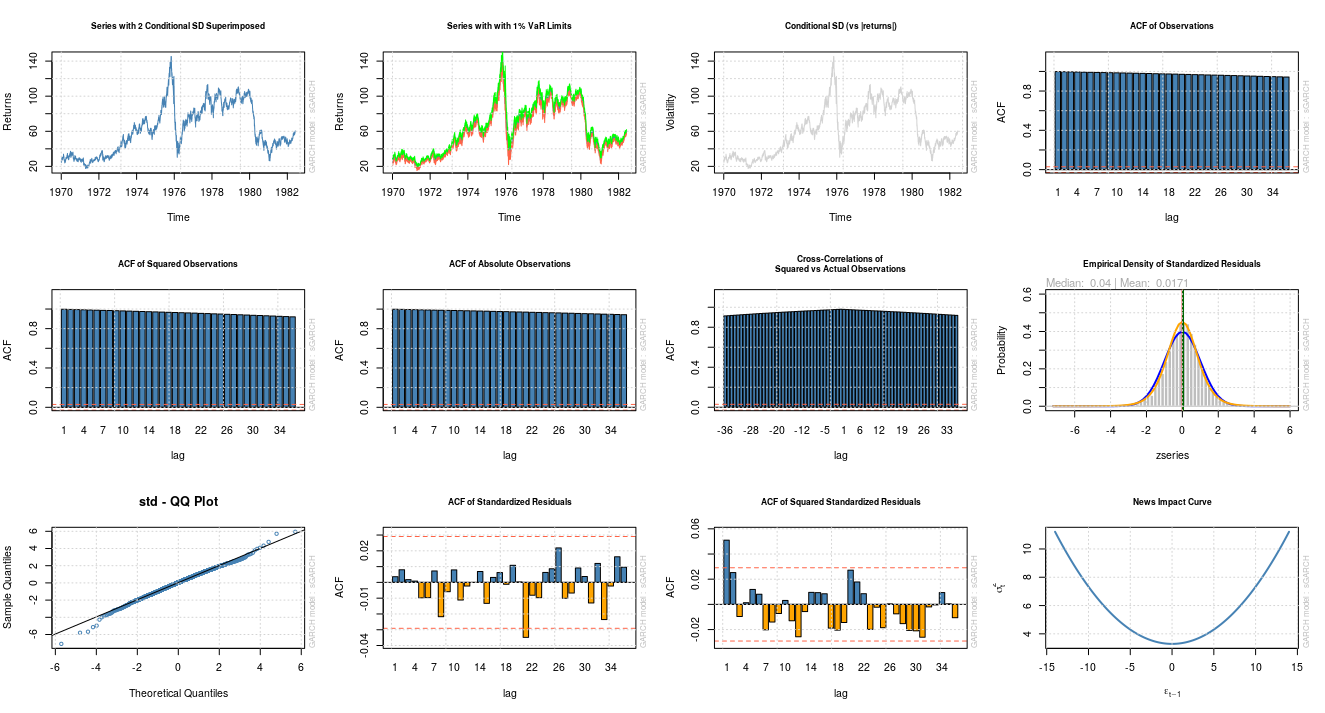
\includegraphics[width=0.85\linewidth]{../Oil-Price-Forecasting/garch}
	\caption{GARCH Plots}
	\label{fig:garch}
\end{figure}

\begin{lstlisting}
#FOR ARMA(0,0)-GARCH(1,1)
Optimal Parameters
------------------------------------
Estimate  Std. Error  t value Pr(>|t|)
mu      49.09642    0.203360 241.4259    0e+00
omega    0.86018    0.172749   4.9793    1e-06
alpha1   0.74558    0.053112  14.0378    0e+00
beta1    0.25342    0.051742   4.8978    1e-06
shape   99.99993   15.542411   6.4340    0e+00

\end{lstlisting}
The shape parameter has p-value = 0<0.05 and hence, is significant. Thus, this model could be significant and a good choice. AIC value = 8.4499 and BIC value = 8.4569. Consider Goodness-of-fit test, we observe that for group 20 and group 40, the p-value<0.05 and hence we can reject the null hypothesis that this model is adequate for this process.


\begin{lstlisting}
## FOR ARMA(1,1)-GARCH(1,1)
        Estimate  Std. Error   t value Pr(>|t|)
mu     25.528948    0.987161   25.8610 0.000000
ar1     1.000000    0.000441 2270.1057 0.000000
ma1    -0.035096    0.014662   -2.3936 0.016685
omega   0.003432    0.001434    2.3938 0.016674
alpha1  0.040423    0.002306   17.5305 0.000000
beta1   0.958576    0.001582  606.0060 0.000000
shape   7.402473    0.732533   10.1053 0.000000


\end{lstlisting}
The shape parameter has p-value = 0<0.05 and hence, is significant. Thus, this model could be significant and a good choice. AIC value =  3.1778 and BIC value = 3.1877.
Considering the Goodness-of-fit test, we observe that for group 20 and group 40, the p-value<0.05 and hence we can reject the null hypothesis that this model is adequate for this process.


The QQ plot for both GARCH series is shown below:
\begin{figure}[h!]
	\centering
	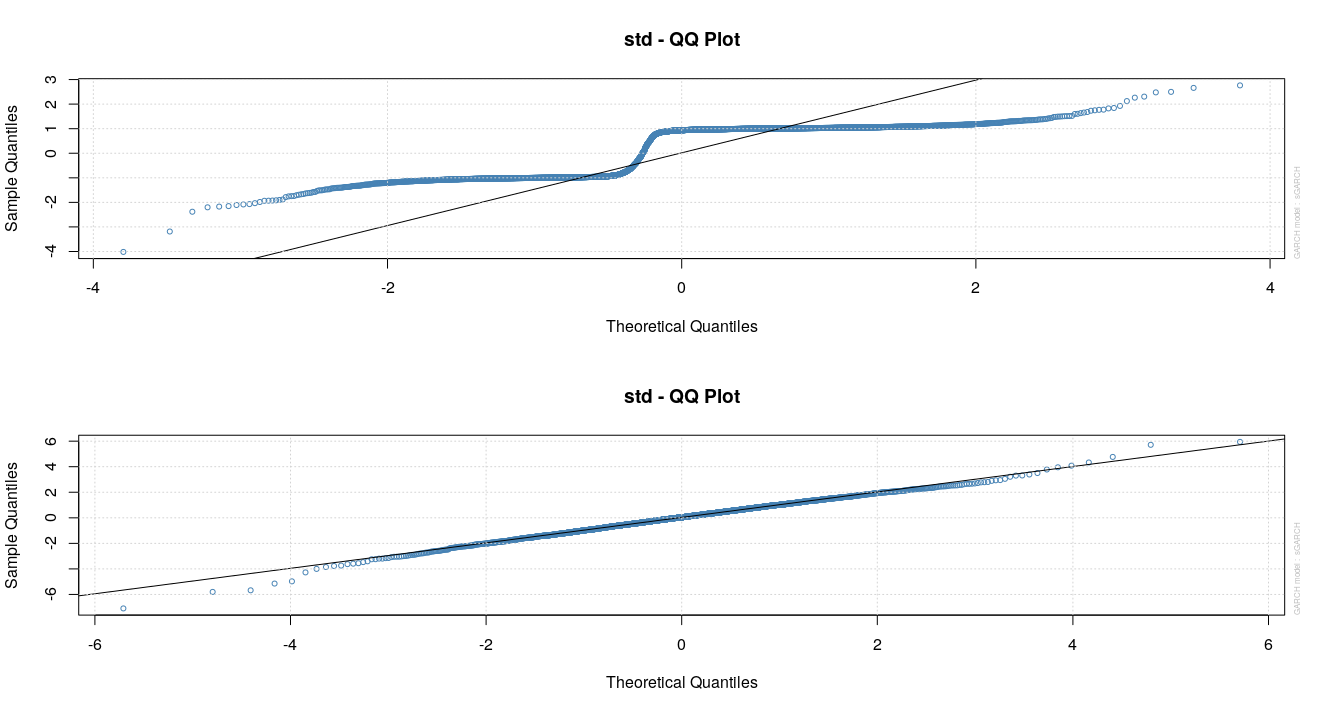
\includegraphics[width=0.95\linewidth]{../Oil-Price-Forecasting/res}
	\caption{QQ plot of Residuals for GARCH}
	\label{fig:res}
\end{figure}

\subsection{Regression with ARIMA errors}
We used two of exogenous variable as enumerated below:
\begin{enumerate}
	\item Google Index cannot help to forecast crude oil prices\cite{yao2017forecasting}
	\item Foreign Currency Exchange Data
\end{enumerate}
dollar-yen-exchange-rate and pound-dollar-exchange-rate for same time period and fitted the regression model. Results for same are reproduced below:

\scriptsize\textbf{for dollar-yen-exchange-rate}
\begin{verbatim}
Series: train 
Regression with ARIMA(2,1,4) errors 
Coefficients:
ar1      ar2     ma1     ma2      ma3     ma4    xreg
-0.8494  -0.6673  0.8001  0.6060  -0.0176  0.0359  0.0033
s.e.   0.1219   0.1416  0.1224  0.1406   0.0231  0.0184  0.0315

sigma^2 estimated as 2.089:  log likelihood=-8103.44
AIC=16222.89   AICc=16222.92   BIC=16274.25

Training set error measures:
ME     RMSE      MAE         MPE     MAPE      MASE          ACF1
Training set 0.007968868 1.444007 1.000096 -0.01138468 1.753645 0.9984232 -0.0002005725
\end{verbatim}
\textbf{for pound-dollar-exchange-rate}
\begin{verbatim}
Series: train 
Regression with ARIMA(3,1,2) errors 
Coefficients:
ar1      ar2      ar3     ma1     ma2   drift    xreg
-0.8000  -0.8916  -0.0372  0.7501  0.8257  0.0081  3.9404
s.e.   0.0105      NaN   0.0161  0.0134     NaN  0.0202  2.0631

sigma^2 estimated as 2.088:  log likelihood=-8102.58
AIC=16221.16   AICc=16221.19   BIC=16272.52

Training set error measures:
ME     RMSE      MAE         MPE     MAPE    MASE         ACF1
Training set -0.0001915481 1.443732 1.001696 -0.02856478 1.756283 1.00002 0.0002121344

\end{verbatim}
\normalsize
Exchange rate data did not improved the accuracy of our model. AIC is still very low. Hence no improvment were observed from adding these two exogeneous data.  
\section{Conclusion \& Discussions}
\subsection{Evaluation criterion} We are using these 3 metrics for evaluating our model. Their respective values are shown is Table: \ref{tab}. The smaller the value -- better for the model. 
\begin{enumerate}
	\item The \textbf{Akaike information criterion (AIC)} is an estimator of out-of-sample prediction error and thereby relative quality of statistical models for a given set of data\cite{ID}.
	\item \textbf{Bayesian information criterion} (BIC) or Schwarz information criterion (also SIC, SBC, SBIC) is a criterion for model selection among a finite set of models; the model with the lowest BIC is preferred.
	\item \textbf{Root Mean Square Error (RMSE)} is the standard deviation of the residuals (prediction errors). Residuals are a measure of how far from the regression line data points are; RMSE is a measure of how spread out these residuals are.
\end{enumerate}
\begin{table}[h!]
	\begin{tabular}{ccccc c}
		\hline
		Model & ARIMA  & SARIMA  & AAR  & GARCH\scriptsize{(ARFIMA(0,0,0)) w/ diff.}\normalsize  & GARCH\scriptsize{(ARFIMA(1,0,1))}\normalsize  \\
		\hline
		AIC	&  16221.44 & 16221.44  & 3376.05 & 8.4499 & \textbf{3.1778} \\
		BIC 	&  16259.94  &16259.94 &3555.81 &4.3472 &\textbf{3.1877} \\	
		RMSE 	& 1.444  &1.444&\textbf{1.130}  & 17.20518 & 6.716708\\\hline
	\end{tabular}
\caption{Evaluation Metrics}\label{tab}
\end{table}

 Essentially, where there is heteroskedasticity, observations do not conform to a linear pattern. Hence, conclusions drawn from a linear model will not be reliable. ARIMA model fails to effectively capture the process being
 followed and subsequent forecasting chosen observations for validation. GARCH model on other hand has best AIC and BIC score and decent RMSE scores too. GARCH processes, being autoregressive, depend on past squared observations and past variances to model for current variance.  Hence, using GARCH for our crude oil forecasting  resulted in a better prediction.
\bibliography{bibo} 
\bibliographystyle{ieeetr}
\appendix
\section*{Code}
The code associated with the experiment, all the data and source code used in preparing this document is available here \texttt{https://github.com/vntkumar8/crude-oil-price}.

\end{document}